% docs/user-guide/main.tex
%
% Grid Calculus — User Guide (memoir class).
% Built via `latexmk -pdf` from build/docs/user-guide/. See docs/README.md
% and docs/CMakeLists.txt.

\documentclass[11pt,oneside,openany]{memoir}

% docs/common/preamble.tex
%
% Shared LaTeX preamble for the gridcalc User Guide (memoir class) and
% Developer Note (book class). Both books \input{} this file.
%
% Phase 10 docs infrastructure. \since 0.10.0 (project versioning).

% --- Encoding -----------------------------------------------------------------
%
% Engine-detection idiom: pdflatex needs `inputenc utf8` + `\DeclareUnicodeCharacter`
% mappings to render Greek / math glyphs the migrated chapters use outside
% math mode; xelatex / lualatex handle Unicode natively via `fontspec`.

\usepackage{iftex}
\ifPDFTeX
  \usepackage[utf8]{inputenc}
  \usepackage[T1]{fontenc}
  \usepackage{textcomp}
\else
  \usepackage{fontspec}
\fi

% --- Math ---------------------------------------------------------------------

\usepackage{amsmath}
\usepackage{amssymb}
\usepackage{amsfonts}
\usepackage{mathtools}

% --- Tables (pandoc emits longtable for markdown tables) ----------------------

\usepackage{longtable}
\usepackage{booktabs}

% Pandoc-emitted body of `--listings` markdown tables expects these.
\providecommand{\toprule}{\hline}
\providecommand{\midrule}{\hline}
\providecommand{\bottomrule}{\hline}

\ifPDFTeX
  % Common Unicode glyphs that pandoc emits in prose (not in math mode) and
  % pdflatex's default declaration set doesn't cover. Map them to math-mode
  % renders so chapters built from the migrated markdown notes compile.
  \DeclareUnicodeCharacter{21D2}{\ensuremath{\Rightarrow}}    % ⇒
  \DeclareUnicodeCharacter{2192}{\ensuremath{\to}}            % →
  \DeclareUnicodeCharacter{2200}{\ensuremath{\forall}}        % ∀
  \DeclareUnicodeCharacter{2208}{\ensuremath{\in}}            % ∈
  \DeclareUnicodeCharacter{2218}{\ensuremath{\circ}}          % ∘
  \DeclareUnicodeCharacter{2202}{\ensuremath{\partial}}       % ∂
  \DeclareUnicodeCharacter{2207}{\ensuremath{\nabla}}         % ∇
  \DeclareUnicodeCharacter{222B}{\ensuremath{\int}}           % ∫
  \DeclareUnicodeCharacter{2248}{\ensuremath{\approx}}        % ≈
  \DeclareUnicodeCharacter{2264}{\ensuremath{\le}}            % ≤
  \DeclareUnicodeCharacter{2265}{\ensuremath{\ge}}            % ≥
  \DeclareUnicodeCharacter{00B7}{\ensuremath{\cdot}}          % ·
  \DeclareUnicodeCharacter{00D7}{\ensuremath{\times}}         % ×
  \DeclareUnicodeCharacter{2212}{-}                            % − (minus)
  \DeclareUnicodeCharacter{00B2}{\ensuremath{^2}}             % ²
  \DeclareUnicodeCharacter{00B3}{\ensuremath{^3}}             % ³
  \DeclareUnicodeCharacter{2074}{\ensuremath{^4}}             % ⁴
  \DeclareUnicodeCharacter{03B1}{\ensuremath{\alpha}}         % α
  \DeclareUnicodeCharacter{03B2}{\ensuremath{\beta}}          % β
  \DeclareUnicodeCharacter{03B3}{\ensuremath{\gamma}}         % γ
  \DeclareUnicodeCharacter{03B5}{\ensuremath{\varepsilon}}    % ε
  \DeclareUnicodeCharacter{03BC}{\ensuremath{\mu}}            % μ
  \DeclareUnicodeCharacter{03C0}{\ensuremath{\pi}}            % π
  \DeclareUnicodeCharacter{03C3}{\ensuremath{\sigma}}         % σ
  \DeclareUnicodeCharacter{03C8}{\ensuremath{\psi}}           % ψ
  \DeclareUnicodeCharacter{0394}{\ensuremath{\Delta}}         % Δ
  \DeclareUnicodeCharacter{03A8}{\ensuremath{\Psi}}           % Ψ
  \DeclareUnicodeCharacter{0398}{\ensuremath{\Theta}}         % Θ
  \DeclareUnicodeCharacter{03B8}{\ensuremath{\theta}}         % θ
  \DeclareUnicodeCharacter{2113}{\ensuremath{\ell}}           % ℓ
  \DeclareUnicodeCharacter{2032}{\ensuremath{'}}              % ′ (prime)
\fi

% --- Code listings ------------------------------------------------------------

\usepackage{listings}
\usepackage{xcolor}

\definecolor{lstkeyword}{RGB}{40,80,160}
\definecolor{lstcomment}{RGB}{96,96,96}
\definecolor{lststring}{RGB}{160,80,40}
\definecolor{lstbg}{RGB}{248,248,248}

% `listings` does not honor `inputenc utf8` inside `\lstinline!...!`, so
% Unicode glyphs that the migrated chapters contain inside code spans
% (`ψ`, `≤`, `²`, etc.) must be mapped via `literate=` substitutions.
% Each substitution maps the UTF-8 glyph to a printable LaTeX form.
\lstset{
    extendedchars=true,
    literate=%
        {²}{{$^2$}}1
        {³}{{$^3$}}1
        {⁴}{{$^4$}}1
        {≤}{{$\leq$}}1
        {≥}{{$\geq$}}1
        {≈}{{$\approx$}}1
        {·}{{$\cdot$}}1
        {×}{{$\times$}}1
        {−}{{-}}1
        {⇒}{{$\Rightarrow$}}1
        {→}{{$\to$}}1
        {∂}{{$\partial$}}1
        {∇}{{$\nabla$}}1
        {∫}{{$\int$}}1
        {∈}{{$\in$}}1
        {∘}{{$\circ$}}1
        {α}{{$\alpha$}}1
        {β}{{$\beta$}}1
        {ε}{{$\varepsilon$}}1
        {μ}{{$\mu$}}1
        {π}{{$\pi$}}1
        {σ}{{$\sigma$}}1
        {ψ}{{$\psi$}}1
        {Δ}{{$\Delta$}}1
        {Ψ}{{$\Psi$}}1
        {Θ}{{$\Theta$}}1
        {θ}{{$\theta$}}1
        {ℓ}{{$\ell$}}1
}

\lstdefinestyle{gridcalcCpp}{
    language=C++,
    basicstyle=\ttfamily\small,
    keywordstyle=\color{lstkeyword}\bfseries,
    commentstyle=\color{lstcomment}\itshape,
    stringstyle=\color{lststring},
    backgroundcolor=\color{lstbg},
    showstringspaces=false,
    breaklines=true,
    breakatwhitespace=true,
    columns=fullflexible,
    keepspaces=true,
    tabsize=2,
    frame=single,
    framesep=4pt,
    framerule=0pt,
    aboveskip=0.6\baselineskip,
    belowskip=0.6\baselineskip,
    morekeywords={
        Field, Grid, Vec3d, Mat3d, Coefficients, FirstDerivative,
        ThirdDerivative, FourthDerivative, IndexPolicy, Periodic,
        ExplicitEuler, RK4, Pairwise, Kahan, ComplexField,
        gridcalc, core, diff, func, solve, spectral, stencil, detail,
        constexpr, noexcept, nullptr, override, final, decltype,
        auto, std, std::size_t, std::complex, std::vector, std::pair,
        std::array
    }
}
\lstset{style=gridcalcCpp}

% --- Hyperlinks (kept conservative for print-friendly PDFs) -------------------

\usepackage[
    colorlinks=true,
    linkcolor=blue!60!black,
    citecolor=blue!60!black,
    urlcolor=blue!60!black,
    pdfborder={0 0 0}
]{hyperref}

% --- File / path typesetting --------------------------------------------------

\usepackage{url}
\providecommand{\path}[1]{\texttt{#1}}

% --- Pandoc-emitted helper commands (the migrated chapters use these) --------

% pandoc emits `\passthrough{...}` for inline code spans under `--listings`.
% Defined as a transparent pass-through.
\providecommand{\passthrough}[1]{#1}

% pandoc emits `\tightlist` immediately inside list environments to suppress
% extra vertical spacing between items.
\providecommand{\tightlist}{\setlength{\itemsep}{0pt}\setlength{\parskip}{0pt}}

% --- Project-local short macros -----------------------------------------------

\providecommand{\gridcalc}{\textsf{gridcalc}}
\providecommand{\Field}{\texttt{Field}}
\providecommand{\Grid}{\texttt{Grid}}
\providecommand{\Order}[1]{\ensuremath{\langle\text{Order}=#1\rangle}}

% Display-math operator helpers used across multiple chapters.
\providecommand{\dd}{\,\mathrm{d}}
\providecommand{\Real}{\mathbb{R}}
\providecommand{\Cplx}{\mathbb{C}}
\providecommand{\norm}[1]{\left\lVert#1\right\rVert}


\title{Grid Calculus \\ \large User Guide}
\author{Byounghak H. Lee}
\date{}

% --- memoir-class layout settings --------------------------------------------

\setstocksize{11in}{8.5in}
\settrimmedsize{11in}{8.5in}{*}
\setlength{\trimtop}{0pt}
\setlength{\trimedge}{0pt}
\settypeblocksize{8in}{6in}{*}
\setlrmargins{*}{*}{1}
\setulmargins{*}{*}{1}
\setheadfoot{\baselineskip}{2\baselineskip}
\setheaderspaces{*}{2\baselineskip}{*}
\checkandfixthelayout

\chapterstyle{section}
\setsecnumdepth{subsection}
\settocdepth{section}

\begin{document}

% --- Front matter -------------------------------------------------------------

\frontmatter

\begin{titlingpage}
    \centering
    \vspace*{2cm}
    {\Huge\bfseries Grid Calculus \par}
    \vspace{0.5cm}
    {\Large User Guide \par}
    \vspace{1.5cm}
    {\large Byounghak H.~Lee \par}
    \vspace{0.5cm}
    {Version \texttt{0.11.0} \par}
    \vfill
    {\small Proprietary; all rights reserved.}
\end{titlingpage}

\tableofcontents*

% --- Main matter --------------------------------------------------------------

\mainmatter

\chapter{Hello grid}
\label{chap:hello-grid}

\textit{This tutorial chapter walks through the operators delivered in
Phases 1--9 with a single end-to-end example. Filled in by Phase 10
Group 5; placeholder until then.}


\chapter{Grid and Laplacian}
\label{chap:grid-and-laplacian}

\textit{Absorbed from \path{docs/user-guide/notes/phase-1-laplacian.md} in
Phase 10 Group 3. Placeholder until migrated.}

\chapter{Gradient and divergence}
\label{chap:gradient-divergence}

\textit{Absorbed from \path{docs/user-guide/notes/phase-2-gradient-divergence.md}
in Phase 10 Group 3. Placeholder until migrated.}

\chapter{Domain integration}
\label{chap:domain-integration}

\begin{quote}
Spec dir:
\passthrough{\lstinline!specs/2026-05-02-phase-3-domain-integration/!}.
Version: \passthrough{\lstinline!0.3.0!}.
\end{quote}

\subsection{What this gives you}\label{what-this-gives-you}

A primitive that turns a scalar \passthrough{\lstinline!Field<double>!}
into a single number --- the discrete integral

\[
\int_{\Omega} f(\mathbf{x})\, dV \;\approx\; h_x h_y h_z \sum_{i,j,k} f_{ijk}
\]

over the periodic Cartesian domain
\passthrough{\lstinline![0, Nx*hx) × [0, Ny*hy) × [0, Nz*hz)!}.

This is the integration backbone the upcoming functional-evaluation API
will sit on (Phase 4).

\subsection{API}\label{api}

Header:
\href{../../../include/gridcalc/func/Integrate.hpp}{\passthrough{\lstinline!include/gridcalc/func/Integrate.hpp!}}.

\begin{lstlisting}[language={C++}]
namespace gridcalc::func {

struct Pairwise {};   // tag selecting pairwise recursive summation
struct Kahan {};      // tag selecting Kahan/Neumaier compensated summation

double integrate(const core::Field<double>& field, Pairwise = {}) noexcept;
double integrate(const core::Field<double>& field, Kahan)        noexcept;

}  // namespace gridcalc::func
\end{lstlisting}

Pick the reducer with a tag:

\begin{itemize}
\tightlist
\item
  \passthrough{\lstinline!integrate(f)!} or
  \passthrough{\lstinline!integrate(f, Pairwise\{\})!} ---
  \textbf{default}. Pairwise recursive summation; rounding error grows
  like \passthrough{\lstinline!O(ε log n)!}. Cheap. Use this unless you
  have a reason not to.
\item
  \passthrough{\lstinline!integrate(f, Kahan\{\})!} --- Neumaier-style
  compensated summation; \textasciitilde bit-perfect accuracy at
  \textasciitilde3-4× cost per element. Use when integrating long sums
  of values whose magnitudes vary by many orders of magnitude.
\end{itemize}

The grid's cell volume \passthrough{\lstinline!hx * hy * hz!} is read
from the input \passthrough{\lstinline!Field!}'s
\passthrough{\lstinline!Grid!} and applied by
\passthrough{\lstinline!integrate()!} itself. You do not multiply by
\passthrough{\lstinline!dV!} yourself.

Periodic wrap is irrelevant here: every grid point is sampled exactly
once, regardless of the input field's
\passthrough{\lstinline!IndexPolicy!}.

\subsection{Worked example}\label{worked-example}

Volume of a 2π cube:

\begin{lstlisting}[language={C++}]
#include <gridcalc/core/Field.hpp>
#include <gridcalc/core/Grid.hpp>
#include <gridcalc/func/Integrate.hpp>

const int N = 32;
const double L = 2.0 * M_PI;
const double h = L / N;

gridcalc::core::Grid grid(N, N, N, gridcalc::core::Vec3d(h, h, h));
gridcalc::core::Field<double> ones(grid, 1.0);

double V = gridcalc::func::integrate(ones);
// V == L*L*L == (2*pi)^3, to machine precision.
\end{lstlisting}

A periodic sinusoid integrates to zero (every axis-orthogonal trig
component sums exactly to zero on equispaced periodic samples):

\begin{lstlisting}[language={C++}]
gridcalc::core::Field<double> psi(grid, [](double x, double y, double z) {
  return std::cos(x) * std::sin(2.0 * y) * std::sin(3.0 * z);
});
double I = gridcalc::func::integrate(psi);   // I ~ 0  (within ~1e-15)
\end{lstlisting}

\subsection{\texorpdfstring{What this does \emph{not} do
(yet)}{What this does not do (yet)}}\label{what-this-does-not-do-yet}

\begin{itemize}
\tightlist
\item
  \textbf{No callable-integrand overload.}
  \passthrough{\lstinline!∫ f(ψ, ∇ψ, ∇²ψ) dV!} for user-supplied
  \passthrough{\lstinline!f!} is the headline of Phase 4 (functional
  evaluation).
\item
  \textbf{No vector-field overload.}
  \passthrough{\lstinline!integrate(Field<Vec3d>)!} arrives when the
  Phase 11+ higher-rank functionals first need it.
\item
  \textbf{No threading.} Phase 3 is single-threaded; Phase 20
  (performance pass) parallelizes the reducer while preserving
  bit-identical output.
\item
  \textbf{No non-periodic boundary handling.} The midpoint formula
  assumes the domain is periodic. Once Phase 18 introduces
  Dirichlet/Neumann fields, endpoint corrections (Euler--Maclaurin,
  Simpson) become relevant.
\end{itemize}

For the why-this-formula-is-correct background --- derivation, error
analysis, references --- see
\href{../../developer-note/notes/phase-3-domain-integration.md}{\passthrough{\lstinline!docs/developer-note/notes/phase-3-domain-integration.md!}}.

\chapter{Functional evaluation}
\label{chap:functional-evaluation}

\begin{quote}
Spec dir:
\passthrough{\lstinline!specs/2026-05-02-phase-4-functional-evaluation/!}.
Version: \passthrough{\lstinline!0.4.0!}.
\end{quote}

\subsection{What this gives you}\label{what-this-gives-you}

A primitive that evaluates a \textbf{functional} of a scalar field ---
an integral of an arbitrary user-supplied integrand
\(f(\psi, \nabla\psi, \nabla^2\psi)\) over the periodic Cartesian
domain:

\[
F[\psi] \;=\; \int_{\Omega} f\bigl(\psi(\mathbf{x}),\, \nabla\psi(\mathbf{x}),\, \nabla^2\psi(\mathbf{x})\bigr)\, dV.
\]

\passthrough{\lstinline!evaluate!} builds on top of Phase 1's
\passthrough{\lstinline!laplacian!}, Phase 2's
\passthrough{\lstinline!gradient!}, and Phase 3's
\passthrough{\lstinline!integrate!}: it materializes whichever
derivatives your \passthrough{\lstinline!f!} actually needs, evaluates
\passthrough{\lstinline!f!} pointwise into a temporary
\passthrough{\lstinline!Field<double>!}, and reduces the result with the
same pairwise / Kahan tag dispatch from Phase 3.

\subsection{API}\label{api}

Header:
\href{../../../include/gridcalc/func/Functional.hpp}{\passthrough{\lstinline!include/gridcalc/func/Functional.hpp!}}.

\begin{lstlisting}[language={C++}]
namespace gridcalc::func {

template <class F, class Tag = Pairwise>
double evaluate(const core::Field<double>& psi, F&& f, Tag tag = {});

}  // namespace gridcalc::func
\end{lstlisting}

Your callable \passthrough{\lstinline!f!} may take \textbf{any one of
three signatures}, picked at compile time by
\passthrough{\lstinline!std::is\_invocable\_r\_v!}:

{\def\LTcaptype{none} % do not increment counter
\begin{longtable}[]{@{}
  >{\raggedright\arraybackslash}p{(\linewidth - 2\tabcolsep) * \real{0.8361}}
  >{\raggedright\arraybackslash}p{(\linewidth - 2\tabcolsep) * \real{0.1639}}@{}}
\toprule\noalign{}
\begin{minipage}[b]{\linewidth}\raggedright
Signature
\end{minipage} & \begin{minipage}[b]{\linewidth}\raggedright
Computes
\end{minipage} \\
\midrule\noalign{}
\endhead
\bottomrule\noalign{}
\endlastfoot
\passthrough{\lstinline!f(double psi)!} & only
\passthrough{\lstinline!ψ!} --- gradient and Laplacian are
\textbf{skipped} \\
\passthrough{\lstinline!f(double psi, const Vec3d\& grad)!} &
\passthrough{\lstinline!ψ!} and \passthrough{\lstinline!∇ψ!} ---
Laplacian is \textbf{skipped} \\
\passthrough{\lstinline!f(double psi, const Vec3d\& grad, double lap)!}
& full triplet \passthrough{\lstinline!ψ!},
\passthrough{\lstinline!∇ψ!}, \passthrough{\lstinline!∇²ψ!} \\
\end{longtable}
}

Return type must be convertible to \passthrough{\lstinline!double!}. The
reducer tag (\passthrough{\lstinline!Pairwise\{\}!} or
\passthrough{\lstinline!Kahan\{\}!}) is forwarded to
\passthrough{\lstinline!func::integrate!}.

\subsection{Worked example: Ginzburg--Landau free
energy}\label{worked-example-ginzburglandau-free-energy}

The Ginzburg--Landau free-energy density is

\[
f_{\mathrm{GL}}(\psi, \nabla\psi) \;=\; \tfrac{1}{2} |\nabla\psi|^2 \;+\; W (\psi^2 - 1)^2,
\]

with \(W\) a positive constant. Note that \(f_{\mathrm{GL}}\) does
\textbf{not} depend on \(\nabla^2\psi\), so writing it with the 2-arg
signature lets \passthrough{\lstinline!evaluate!} skip the Laplacian
computation.

\subsubsection{Setup}\label{setup}

\begin{lstlisting}[language={C++}]
#include <cmath>
#include <gridcalc/core/EigenAliases.hpp>
#include <gridcalc/core/Field.hpp>
#include <gridcalc/core/Grid.hpp>
#include <gridcalc/func/Functional.hpp>

using gridcalc::core::Field;
using gridcalc::core::Grid;
using gridcalc::core::Vec3d;
using gridcalc::func::evaluate;

constexpr double kPi = 3.14159265358979323846;

const int N = 64;
const double L = 2.0 * kPi;
const double h = L / N;
const double W = 1.0;

Grid grid(N, N, N, Vec3d(h, h, h));
Field<double> psi(grid, [](double x, double y, double z) {
  return std::sin(x) * std::sin(y) * std::sin(z);
});
\end{lstlisting}

\subsubsection{The integrand}\label{the-integrand}

\begin{lstlisting}[language={C++}]
auto gl_density = [W](double p, const Vec3d& g) {
  const double dpsi2 = p * p - 1.0;
  return 0.5 * g.squaredNorm() + W * dpsi2 * dpsi2;
};
\end{lstlisting}

\subsubsection{Evaluate}\label{evaluate}

\begin{lstlisting}[language={C++}]
const double F = evaluate(psi, gl_density);
\end{lstlisting}

For this \passthrough{\lstinline!ψ!} with
\passthrough{\lstinline!W = 1!}, the analytical reference is
\(F = (3/2)\pi^3 + (411/64)\pi^3 = (507/64)\pi^3 \approx 245.62\). At
\passthrough{\lstinline!N = 64!}, \passthrough{\lstinline!evaluate!}
matches this to better than 0.5\% relative error; the discrete error is
dominated by the squared-gradient term and converges at order 2 in \(h\)
(verified by
\href{../../../test/functional_test.cpp}{\passthrough{\lstinline!test/functional\_test.cpp!}}'s
\passthrough{\lstinline!GinzburgLandauSecondOrderConvergence!} test).

For the why-this-formula-converges-at-order-2 background --- derivation,
error analysis, references --- see
\href{../../developer-note/notes/phase-4-functional-evaluation.md}{\passthrough{\lstinline!docs/developer-note/notes/phase-4-functional-evaluation.md!}}.

\subsection{\texorpdfstring{What this does \emph{not} do
(yet)}{What this does not do (yet)}}\label{what-this-does-not-do-yet}

\begin{itemize}
\tightlist
\item
  \textbf{No vector-field functionals.}
  \passthrough{\lstinline!evaluate(Field<Vec3d>, …)!} arrives in Phase
  11+ when the higher-rank functionals first need it.
\item
  \textbf{No higher-order derivatives in \passthrough{\lstinline!f!}.}
  Phase 6 adds biharmonic and mixed partials; Phase 11 adds
  up-to-4th-order gradients.
\item
  \textbf{No variational derivative \passthrough{\lstinline!δF/δψ!}.}
  Phase 12 (CH demo) adds closed-form variational derivatives where they
  are needed.
\item
  \textbf{No fused-loop optimization.}
  \passthrough{\lstinline!evaluate!} materializes intermediate Fields
  for \passthrough{\lstinline!∇ψ!} and/or \passthrough{\lstinline!∇²ψ!}.
  Phase 11+ replaces this with expression-template fusion.
\end{itemize}

\subsection{Quick reference: which arity to
pick}\label{quick-reference-which-arity-to-pick}

\begin{itemize}
\tightlist
\item
  Integrand depends only on \passthrough{\lstinline!ψ!} (e.g.,
  \passthrough{\lstinline!∫ ψ² dV!},
  \passthrough{\lstinline!∫ W(ψ²-1)² dV!}): use
  \passthrough{\lstinline!f(double)!}. Saves both stencil computations.
\item
  Integrand uses \passthrough{\lstinline!∇ψ!} (e.g., the gradient term
  of any GL-style energy): use
  \passthrough{\lstinline!f(double, const Vec3d\&)!}. Saves the
  Laplacian.
\item
  Integrand uses \passthrough{\lstinline!∇²ψ!} (Cahn--Hilliard kernel,
  surface-tension derivatives): use
  \passthrough{\lstinline!f(double, const Vec3d\&, double)!}.
\end{itemize}

\chapter{Explicit-Euler diffusion}
\label{chap:explicit-euler}

\textit{Absorbed from \path{docs/user-guide/notes/phase-5-explicit-euler.md}
in Phase 10 Group 3. Placeholder until migrated.}

\chapter{RK4 time integration}
\label{chap:rk4-time-integration}

\begin{quote}
Spec dir:
\passthrough{\lstinline!specs/2026-05-02-phase-6-rk4-integrator/!}.
Version: \passthrough{\lstinline!0.6.0!}.
\end{quote}

\subsection{What this gives you}\label{what-this-gives-you}

A higher-order time integrator (classic 4-stage Runge--Kutta) and a
\textbf{generic dispatcher} that lets you pick which integrator to use:

\begin{lstlisting}[language={C++}]
solve::integrate(psi, rhs, dt, n_steps, IntegratorTag{});
\end{lstlisting}

with \passthrough{\lstinline!IntegratorTag!} being either
\passthrough{\lstinline!solve::ExplicitEuler!} (Phase 5) or
\passthrough{\lstinline!solve::RK4!} (new in Phase 6).

\passthrough{\lstinline!solve::diffuse!} is now templated on the
integrator tag so you can swap between Euler and RK4 with one extra
argument:

\begin{lstlisting}[language={C++}]
solve::diffuse(psi, D, dt, n_steps);                    // Euler (default)
solve::diffuse(psi, D, dt, n_steps, solve::RK4{});      // RK4
\end{lstlisting}

RK4 is \textbf{more accurate} at the same \passthrough{\lstinline!dt!}
(4 orders better --- the time-error per step is
\passthrough{\lstinline!O(dt\^5)!} vs Euler's
\passthrough{\lstinline!O(dt\^2)!}) and has a \textbf{larger stability
bound} for the heat equation
(\passthrough{\lstinline!D dt sum(1/h\_a\^2) ≤ 0.6963!} vs Euler's
\passthrough{\lstinline!0.5!}). The cost is 4 RHS evaluations per step
instead of 1.

\subsection{API}\label{api}

Headers:
\href{../../../include/gridcalc/solve/Integrator.hpp}{\passthrough{\lstinline!include/gridcalc/solve/Integrator.hpp!}}
(one-stop aggregator),
\href{../../../include/gridcalc/solve/ExplicitEuler.hpp}{\passthrough{\lstinline!include/gridcalc/solve/ExplicitEuler.hpp!}},
\href{../../../include/gridcalc/solve/RK4.hpp}{\passthrough{\lstinline!include/gridcalc/solve/RK4.hpp!}},
\href{../../../include/gridcalc/solve/Diffusion.hpp}{\passthrough{\lstinline!include/gridcalc/solve/Diffusion.hpp!}}.

\begin{lstlisting}[language={C++}]
namespace gridcalc::solve {

// Integrator tag types -- empty structs that carry compile-time properties.
struct ExplicitEuler { static constexpr double diffusionCFLLimit = 0.5;    };
struct RK4           { static constexpr double diffusionCFLLimit = 0.6963; };

// Generic dispatcher (overloaded on tag).
template <class Rhs>
void integrate(core::Field<double>& psi, Rhs&& rhs, double dt, int n_steps, ExplicitEuler);

template <class Rhs>
void integrate(core::Field<double>& psi, Rhs&& rhs, double dt, int n_steps, RK4);

// Phase-5 thin wrapper -- equivalent to integrate(..., ExplicitEuler{}).
template <class Rhs>
void explicitEuler(core::Field<double>& psi, Rhs&& rhs, double dt, int n_steps);

// Diffusion driver -- now templated on integrator tag.
template <class Integrator = ExplicitEuler>
void diffuse(core::Field<double>& psi, double D, double dt, int n_steps,
             Integrator tag = {});

}  // namespace gridcalc::solve
\end{lstlisting}

\subsubsection{Picking an integrator}\label{picking-an-integrator}

{\def\LTcaptype{none} % do not increment counter
\begin{longtable}[]{@{}
  >{\raggedright\arraybackslash}p{(\linewidth - 2\tabcolsep) * \real{0.8088}}
  >{\raggedright\arraybackslash}p{(\linewidth - 2\tabcolsep) * \real{0.1912}}@{}}
\toprule\noalign{}
\begin{minipage}[b]{\linewidth}\raggedright
Want
\end{minipage} & \begin{minipage}[b]{\linewidth}\raggedright
Use
\end{minipage} \\
\midrule\noalign{}
\endhead
\bottomrule\noalign{}
\endlastfoot
Simplest, smallest per-step cost &
\passthrough{\lstinline!ExplicitEuler\{\}!} (Phase 5 default) \\
Best accuracy per step & \passthrough{\lstinline!RK4\{\}!} \\
Larger time step (closer to RK4's \passthrough{\lstinline!\~1.39×!}
looser CFL) & \passthrough{\lstinline!RK4\{\}!} \\
Pure linear / Hamiltonian / oscillatory dynamics &
\passthrough{\lstinline!RK4\{\}!} (lower phase error) \\
One-pass throwaway integration of a smooth IC & Either; default Euler is
fine \\
\end{longtable}
}

Both integrators take the same RHS callable signature:
\passthrough{\lstinline!Field<double> rhs(const Field<double>\&)!}.
SFINAE-validates; mismatch trips a
\passthrough{\lstinline!static\_assert!}.

\subsubsection{CFL stability check}\label{cfl-stability-check}

\passthrough{\lstinline!solve::diffuse!} validates the von-Neumann bound
\passthrough{\lstinline!D · dt · sum\_a(1/h\_a\^2) ≤ Tag::diffusionCFLLimit!}
before integration begins and throws
\passthrough{\lstinline!std::invalid\_argument!} if violated. The error
message names the integrator type, the offending values, and the
applicable limit.

\passthrough{\lstinline!solve::integrate!} and
\passthrough{\lstinline!solve::explicitEuler!} do \textbf{not} check CFL
--- they're generic over the RHS, which means they cannot know the
relevant stability bound. If you call them directly with a custom RHS,
you own the stability argument.

\subsection{Worked example: heat equation with
RK4}\label{worked-example-heat-equation-with-rk4}

\begin{lstlisting}[language={C++}]
#include <cmath>
#include <gridcalc/core/Field.hpp>
#include <gridcalc/core/Grid.hpp>
#include <gridcalc/solve/Diffusion.hpp>
#include <gridcalc/solve/Integrator.hpp>

using gridcalc::core::Field;
using gridcalc::core::Grid;
using gridcalc::core::Vec3d;
using gridcalc::solve::diffuse;
using gridcalc::solve::RK4;

constexpr double kPi = 3.14159265358979323846;

const int N = 32;
const double L = 2.0 * kPi;
const double h = L / N;
const double D = 0.1;
const double dt = 0.05;
const int n_steps = 100;

Grid grid(N, N, N, Vec3d(h, h, h));

Field<double> psi(grid, [](double x, double y, double z) {
  return std::sin(x) * std::sin(y) * std::sin(z);
});

// One-line switch from Euler to RK4: pass the integrator tag.
diffuse(psi, D, dt, n_steps, RK4{});

// psi now matches the analytical exp(-3 D T) sin(x) sin(y) sin(z) to
// within ~0.5% relative max-norm error -- 10x tighter than Phase 5's
// Euler at the same parameters.
\end{lstlisting}

\subsection{Worked example: custom RHS (no CFL
gating)}\label{worked-example-custom-rhs-no-cfl-gating}

\begin{lstlisting}[language={C++}]
#include <gridcalc/diff/Laplacian.hpp>
#include <gridcalc/solve/Integrator.hpp>

// Reaction-diffusion: dpsi/dt = D laplacian(psi) - k psi
auto rhs = [D, k](const Field<double>& f) {
  Field<double> out = gridcalc::diff::laplacian(f);
  const std::size_t N_ = out.getSize();
  double* o = out.data();
  const double* p = f.data();
  for (std::size_t n = 0; n < N_; ++n) {
    o[n] = D * o[n] - k * p[n];
  }
  return out;
};

// RK4 makes this much more accurate than Euler at the same dt.
gridcalc::solve::integrate(psi, rhs, dt, n_steps, gridcalc::solve::RK4{});
\end{lstlisting}

\subsection{\texorpdfstring{What this does \emph{not} do
(yet)}{What this does not do (yet)}}\label{what-this-does-not-do-yet}

\begin{itemize}
\tightlist
\item
  \textbf{No adaptive time stepping.} Embedded RK methods (RK4(5),
  Dormand--Prince) arrive only if a downstream phase needs them.
\item
  \textbf{No symplectic / structure-preserving integrators.} Heat
  equation is dissipative; symplectic schemes are for Hamiltonian flows.
\item
  \textbf{No multistep methods (Adams--Bashforth, BDF).} Implicit BDF
  arrives in Phase 19.
\item
  \textbf{No persistent scratch pool for RK4.} Each step allocates
  \textasciitilde6 fields; Phase 20 swaps in a reusable scratch buffer.
\item
  \textbf{Boundary conditions: still periodic-only.} Phase 18's
  Dirichlet/Neumann policies will need their own integrator-test
  coverage; tracked in \passthrough{\lstinline!STATUS.md!} ``Open /
  deferred items.''
\end{itemize}

For the why-RK4-is-order-4 derivation and the stability-bound
calculation, see
\href{../../developer-note/notes/phase-6-rk4-integrator.md}{\passthrough{\lstinline!docs/developer-note/notes/phase-6-rk4-integrator.md!}}.

\chapter{Higher-order accuracy stencils}
\label{chap:higher-order-stencils}

\textit{Absorbed from
\path{docs/user-guide/notes/phase-7-higher-order-stencils.md} in Phase
10 Group 3. Placeholder until migrated.}

\chapter{Higher-order spatial derivatives}
\label{chap:higher-order-spatial-derivatives}

\begin{quote}
Spec dir:
\passthrough{\lstinline!specs/2026-05-02-phase-8-higher-order-derivatives/!}.
Version: \passthrough{\lstinline!0.8.0!}.
\end{quote}

\subsection{What this gives you}\label{what-this-gives-you}

Every distinct scalar partial derivative on the periodic Cartesian grid
up to total rank 4, plus the biharmonic operator \(\nabla^4\). Each
operator is templated on accuracy \passthrough{\lstinline!Order = 2!}
(default) or \passthrough{\lstinline!Order = 4!}, mirroring Phase 7's
switching mechanism on \passthrough{\lstinline!laplacian!},
\passthrough{\lstinline!gradient!},
\passthrough{\lstinline!divergence!}.

\begin{lstlisting}[language={C++}]
diff::dxx(psi);              // ∂²ψ/∂x² (rank 2, order 2 default)
diff::dxy<4>(psi);           // ∂²ψ/∂x∂y (rank 2, order 4)
diff::d3dx2dy(psi);          // ∂³ψ/∂x²∂y (rank 3)
diff::d3dxdydz<4>(psi);      // ∂³ψ/∂x∂y∂z (rank 3, order 4)
diff::d4dx2dy2(psi);         // ∂⁴ψ/∂x²∂y² (rank 4)
diff::d4dx2dydz<4>(psi);     // ∂⁴ψ/∂x²∂y∂z (rank 4, order 4)
diff::biharmonic(psi);       // ∇⁴ψ (rank 4, contracted)
diff::d4(psi);               // alias for biharmonic — same result
\end{lstlisting}

\subsection{Naming convention}\label{naming-convention}

\passthrough{\lstinline!d<rank>d<axis-with-exponent>...!}. The rules:

\begin{enumerate}
\def\labelenumi{\arabic{enumi}.}
\tightlist
\item
  \textbf{Total rank} appears once after the leading
  \passthrough{\lstinline!d!} (e.g., \passthrough{\lstinline!d3!} for a
  rank-3 partial).
\item
  \textbf{Each distinct axis} is listed in \textbf{lexicographic order}
  (\passthrough{\lstinline!x!} → \passthrough{\lstinline!y!} →
  \passthrough{\lstinline!z!}), with its \textbf{exponent} (the
  multiplicity of differentiation along that axis). Exponent of
  \passthrough{\lstinline!1!} is omitted.
\item
  Concatenated as one identifier; no separators, lowercase.
\end{enumerate}

{\def\LTcaptype{none} % do not increment counter
\begin{longtable}[]{@{}
  >{\raggedright\arraybackslash}p{(\linewidth - 2\tabcolsep) * \real{0.7541}}
  >{\raggedright\arraybackslash}p{(\linewidth - 2\tabcolsep) * \real{0.2459}}@{}}
\toprule\noalign{}
\begin{minipage}[b]{\linewidth}\raggedright
Math notation
\end{minipage} & \begin{minipage}[b]{\linewidth}\raggedright
Function name
\end{minipage} \\
\midrule\noalign{}
\endhead
\bottomrule\noalign{}
\endlastfoot
\(\partial^2 \psi / \partial x^2\) & \passthrough{\lstinline!dxx!} \\
\(\partial^2 \psi / \partial y^2\) & \passthrough{\lstinline!dyy!} \\
\(\partial^2 \psi / \partial z^2\) & \passthrough{\lstinline!dzz!} \\
\(\partial^2 \psi / \partial x \partial y\) &
\passthrough{\lstinline!dxy!} \\
\(\partial^2 \psi / \partial x \partial z\) &
\passthrough{\lstinline!dxz!} \\
\(\partial^2 \psi / \partial y \partial z\) &
\passthrough{\lstinline!dyz!} \\
\(\partial^3 \psi / \partial x^3\) & \passthrough{\lstinline!d3dx3!} \\
\(\partial^3 \psi / \partial x^2 \partial y\) &
\passthrough{\lstinline!d3dx2dy!} \\
\(\partial^3 \psi / \partial x \partial y^2\) &
\passthrough{\lstinline!d3dxdy2!} \\
\(\partial^3 \psi / \partial x \partial y \partial z\) &
\passthrough{\lstinline!d3dxdydz!} \\
\(\partial^4 \psi / \partial x^4\) & \passthrough{\lstinline!d4dx4!} \\
\(\partial^4 \psi / \partial x^3 \partial y\) &
\passthrough{\lstinline!d4dx3dy!} \\
\(\partial^4 \psi / \partial x^2 \partial y^2\) &
\passthrough{\lstinline!d4dx2dy2!} \\
\(\partial^4 \psi / \partial x^2 \partial y \partial z\) &
\passthrough{\lstinline!d4dx2dydz!} \\
\(\nabla^4 \psi\) (contracted) & \passthrough{\lstinline!biharmonic!}
\emph{or} \passthrough{\lstinline!d4!} \\
\end{longtable}
}

A single shorthand like \passthrough{\lstinline!d4!} (no axis suffix)
denotes the \textbf{contracted scalar operator} at that rank ---
\(\nabla^4\) for \passthrough{\lstinline!d4!}. Phase 8 ships only the
even-rank shorthand \passthrough{\lstinline!d4!} because \$\nabla\^{}2 =
\$ Laplacian already has the familiar name
\passthrough{\lstinline!laplacian!} and isn't being renamed.

\subsection{API}\label{api}

Headers under
\href{../../../include/gridcalc/diff/}{\passthrough{\lstinline!include/gridcalc/diff/!}}:

{\def\LTcaptype{none} % do not increment counter
\begin{longtable}[]{@{}
  >{\raggedright\arraybackslash}p{(\linewidth - 2\tabcolsep) * \real{0.2243}}
  >{\raggedright\arraybackslash}p{(\linewidth - 2\tabcolsep) * \real{0.7757}}@{}}
\toprule\noalign{}
\begin{minipage}[b]{\linewidth}\raggedright
Header
\end{minipage} & \begin{minipage}[b]{\linewidth}\raggedright
Operators
\end{minipage} \\
\midrule\noalign{}
\endhead
\bottomrule\noalign{}
\endlastfoot
\passthrough{\lstinline!MixedPartial.hpp!} &
\passthrough{\lstinline!dxx!}, \passthrough{\lstinline!dyy!},
\passthrough{\lstinline!dzz!}, \passthrough{\lstinline!dxy!},
\passthrough{\lstinline!dxz!}, \passthrough{\lstinline!dyz!} (6 rank-2
partials) \\
\passthrough{\lstinline!ThirdOrder.hpp!} & 10 rank-3 partials
(\passthrough{\lstinline!d3dx3!}, \ldots,
\passthrough{\lstinline!d3dxdydz!}) \\
\passthrough{\lstinline!FourthOrder.hpp!} & 15 rank-4 partials
(\passthrough{\lstinline!d4dx4!}, \ldots,
\passthrough{\lstinline!d4dxdydz2!}) \\
\passthrough{\lstinline!Biharmonic.hpp!} &
\passthrough{\lstinline!biharmonic!}, \passthrough{\lstinline!d4!}
alias \\
\end{longtable}
}

Every function has the same signature shape:

\begin{lstlisting}[language={C++}]
template <int Order = 2>
inline core::Field<double> NAME(const core::Field<double>& psi);
\end{lstlisting}

\passthrough{\lstinline!Order!} must be a supported even integer
(\passthrough{\lstinline!2!} or \passthrough{\lstinline!4!} at Phase 8).
Calling e.g.~\passthrough{\lstinline!d3dx2dy<3>(psi)!} triggers a
\textbf{compile error} at the call site (the underlying primary template
is intentionally undefined), not a silent zero-stencil bug.

\subsubsection{Stencil radius and per-point
cost}\label{stencil-radius-and-per-point-cost}

{\def\LTcaptype{none} % do not increment counter
\begin{longtable}[]{@{}
  >{\raggedright\arraybackslash}p{(\linewidth - 6\tabcolsep) * \real{0.2321}}
  >{\raggedright\arraybackslash}p{(\linewidth - 6\tabcolsep) * \real{0.2054}}
  >{\raggedright\arraybackslash}p{(\linewidth - 6\tabcolsep) * \real{0.2054}}
  >{\raggedright\arraybackslash}p{(\linewidth - 6\tabcolsep) * \real{0.3571}}@{}}
\toprule\noalign{}
\begin{minipage}[b]{\linewidth}\raggedright
Operator family
\end{minipage} & \begin{minipage}[b]{\linewidth}\raggedright
Order 2 radius / axis
\end{minipage} & \begin{minipage}[b]{\linewidth}\raggedright
Order 4 radius / axis
\end{minipage} & \begin{minipage}[b]{\linewidth}\raggedright
Per-point reads (worst case at rank 4)
\end{minipage} \\
\midrule\noalign{}
\endhead
\bottomrule\noalign{}
\endlastfoot
Single-axis (\passthrough{\lstinline!d3dx3!},
\passthrough{\lstinline!d4dx4!}) & 2 / 0 / 0 & 3 / 0 / 0 &
\passthrough{\lstinline!5!} (order 2) → \passthrough{\lstinline!7!}
(order 4) \\
Two-axis (\passthrough{\lstinline!d3dx2dy!},
\passthrough{\lstinline!d4dx2dy2!}) & 2 / 1 / 0 → 2 / 2 / 0 & 3 / 2 / 0
→ 3 / 3 / 0 & up to \passthrough{\lstinline!25!} (order 2) →
\passthrough{\lstinline!49!} (order 4) \\
Three-axis (\passthrough{\lstinline!d3dxdydz!},
\passthrough{\lstinline!d4dx2dydz!}) & various & various & up to
\passthrough{\lstinline!27!} (order 2) → \passthrough{\lstinline!147!}
(order 4) \\
\passthrough{\lstinline!biharmonic!} & 6 stencils combined & 6 stencils
combined & order 2: \textasciitilde{}\passthrough{\lstinline!27!}; order
4: \textasciitilde{}\passthrough{\lstinline!81!} \\
\end{longtable}
}

Per-axis \(1/h_a^{N_a}\) scaling means \textbf{anisotropic per-axis
spacing} is handled by the existing \passthrough{\lstinline!Field!}'s
\passthrough{\lstinline!Vec3d \{hx, hy, hz\}!} without any weight-table
modification.

\subsection{\texorpdfstring{Worked example: \(\nabla^4\) on a sinusoidal
eigenfunction}{Worked example: \textbackslash nabla\^{}4 on a sinusoidal eigenfunction}}\label{worked-example-nabla4-on-a-sinusoidal-eigenfunction}

For \(\psi(\mathbf{x}) = \sin(\mathbf{k}\cdot\mathbf{x})\) on the
periodic \([0, 2\pi)^3\) box, the biharmonic recovers
\(|\mathbf{k}|^4\):

\[\nabla^4 \psi = |\mathbf{k}|^4\,\psi.\]

Numerically:

\begin{lstlisting}[language={C++}]
#include <cmath>
#include <gridcalc/core/EigenAliases.hpp>
#include <gridcalc/core/Field.hpp>
#include <gridcalc/core/Grid.hpp>
#include <gridcalc/diff/Biharmonic.hpp>

using gridcalc::core::Field;
using gridcalc::core::Grid;
using gridcalc::core::Vec3d;
using gridcalc::diff::biharmonic;

constexpr double kPi = 3.14159265358979323846;

const int N = 64;
const double L = 2.0 * kPi;
const double h = L / N;

Grid grid(N, N, N, Vec3d(h, h, h));
Field<double> psi(grid, [](double x, double y, double z) {
  return std::sin(x + 2.0 * y + z);                    // k = (1, 2, 1), |k|² = 6
});

Field<double> bh_o2 = biharmonic<2>(psi);              // ~6% relative error at N=64
Field<double> bh_o4 = biharmonic<4>(psi);              // ~3e-3 relative error at N=64

// bh ≈ |k|⁴ * psi = 36 * psi
\end{lstlisting}

For the same accuracy, order 4 lets you stay on a coarser grid and saves
substantial memory in 3D (each grid refinement is 8× the storage).

\subsection{Combining with Phase 1--7
operators}\label{combining-with-phase-17-operators}

The Phase 8 operators are first-class members of
\passthrough{\lstinline!gridcalc::diff!} and compose with everything
from Phases 1--7 by ordinary function composition. Examples:

\begin{itemize}
\tightlist
\item
  A \textbf{biharmonic regularizer} on a free-energy functional written
  through Phase 4's \passthrough{\lstinline!func::evaluate!}: pass
  \passthrough{\lstinline![](const Field\& f) \{ return biharmonic<4>(f); \}!}
  as the integrand.
\item
  A \textbf{fourth-order PDE driver} through Phase 6's
  \passthrough{\lstinline!solve::integrate!}: build the RHS callable
  using \passthrough{\lstinline!diff::biharmonic<4>!} plus any other
  Phase 8 partials.
\end{itemize}

\subsection{\texorpdfstring{What this does \emph{not} do
(yet)}{What this does not do (yet)}}\label{what-this-does-not-do-yet}

\begin{itemize}
\tightlist
\item
  \textbf{No order ≥ 6 stencils.} Same call as Phase 7 --- needs a
  Fornberg generator the project has not yet built.
\item
  \textbf{No order-3 / asymmetric stencils.} Symmetric central
  differences have even truncation orders only.
\item
  \textbf{No vector- or tensor-valued partial-derivative entry points.}
  The Phase 8 family is
  \passthrough{\lstinline!Field<double> → Field<double>!} only.
  Up-to-4th-order \emph{gradient} (Phase 11) and vector / tensor fields
  (Phase 13/14) own those.
\item
  \textbf{No spectral verification.} Phase 9 adds the FFT cross-check on
  every Phase 8 operator.
\item
  \textbf{No non-orthogonal Bravais grids.} Phase 15 ---
  cross-derivative terms appear and the per-axis-independent stencil
  structure breaks down.
\item
  \textbf{No runtime-order or runtime-multi-index dispatch.}
  Compile-time only; add a thin wrapper layer downstream if
  config-file-driven dispatch is needed.
\end{itemize}

For the Taylor-matching derivation of the 3rd- and 4th-derivative weight
tables, the outer-product reasoning behind the multi-axis stencils, and
the design rationale for the d-prefix naming convention, see
\href{../../developer-note/notes/phase-8-higher-order-derivatives.md}{\passthrough{\lstinline!docs/developer-note/notes/phase-8-higher-order-derivatives.md!}}.

\chapter{Spectral verification}
\label{chap:spectral-verification-ug}

\textit{Absorbed from
\path{docs/user-guide/notes/phase-9-spectral-verification.md} in Phase
10 Group 3. Placeholder until migrated.}

\chapter{Higher-order functionals}
\label{chap:higher-order-functional}

\begin{quote}
Spec dir:
\passthrough{\lstinline!specs/2026-05-03-phase-11-higher-order-functional/!}.
Version: \passthrough{\lstinline!0.11.0!}.
\end{quote}

\subsection{What this gives you}\label{phase11-what}

A fourth callable arity for \passthrough{\lstinline!gridcalc::func::evaluate!}
that exposes the contracted-scalar biharmonic
\(\nabla^4\psi\) in the integrand. Together with the three arities from
Phase 4, the supported densities are

\begin{lstlisting}[language={C++}]
double f(double psi);                                                            // arity 1
double f(double psi, const Vec3d& grad);                                         // arity 2
double f(double psi, const Vec3d& grad, double lap);                             // arity 3
double f(double psi, const Vec3d& grad, double lap, double biharm);              // arity 4 (new)
\end{lstlisting}

\passthrough{\lstinline!evaluate!} picks the longest matching arity at
compile time and materializes only the derivatives that arity needs.
At arity 4 it materializes \passthrough{\lstinline!gradient(psi)!},
\passthrough{\lstinline!laplacian(psi)!}, and
\passthrough{\lstinline!biharmonic(psi)!} (Phase 8's fused six-term
direct stencil), then forms the integrand pointwise and reduces with
\passthrough{\lstinline!func::integrate!}. The new fourth argument is a
plain \passthrough{\lstinline!double!} per grid point --- it is the
return type of \passthrough{\lstinline!diff::biharmonic!}.

\textbf{Out of scope at Phase 11.} Rank-3 and rank-4 tensor-valued
derivative arguments (the full \(\nabla^3\psi\), \(\nabla^4\psi\)
objects) are deferred to Phase 13/14, where the tensor type and the
contraction expression-template machinery will land together. If your
density only needs the contracted scalars (Laplacian and biharmonic),
the Phase 11 surface is enough.

\subsection{API}\label{phase11-api}

The signature of \passthrough{\lstinline!evaluate!} is unchanged --- the
new arity is a fourth branch in the existing dispatch ladder. Tag
forwarding to \passthrough{\lstinline!func::integrate!} works as before:

\begin{lstlisting}[language={C++}]
namespace gridcalc::func {

template <class F, class Tag = Pairwise>
double evaluate(const core::Field<double>& psi, F&& f, Tag tag = {});

}  // namespace gridcalc::func
\end{lstlisting}

The compile-time error message for an unsupported callable enumerates
all four arities.

\subsection{Worked example: phase-field-crystal free
energy}\label{phase11-pfc}

The phase-field-crystal (PFC) functional is the canonical use case for
this phase. It models an ordered solid as the minimum of a free
energy whose derivative kernel \((q_0^2 + \nabla^2)^2\) selects a
preferred wavelength near \(q_0\):

\[
F[\psi] \;=\; \int \Big[\tfrac{1}{2}\,\psi\,\big[(q_0^2 + \nabla^2)^2 - \epsilon\big]\,\psi \;+\; \tfrac{1}{4}\,\psi^4\Big]\,\dd V.
\]

Expanding \((q_0^2 + \nabla^2)^2 = q_0^4 + 2q_0^2\nabla^2 + \nabla^4\)
gives the four-term form the integrand lambda implements:

\[
F[\psi] \;=\; \int \Big[\tfrac{1}{2}(q_0^4 - \epsilon)\,\psi^2 \;+\; q_0^2\,\psi\,\nabla^2\psi \;+\; \tfrac{1}{2}\,\psi\,\nabla^4\psi \;+\; \tfrac{1}{4}\,\psi^4\Big]\,\dd V.
\]

For the manufactured solution \(\psi(\mathbf{x}) = \sin x\,\sin y\,\sin z\)
on the periodic box \([0, 2\pi)^3\), the derivative chain is
\(\nabla^2\psi = -3\psi\), \(\nabla^4\psi = 9\psi\), and the relevant
integrals are
\(\int\psi^2 = \pi^3\), \(\int\psi^4 = \tfrac{27\pi^3}{64}\).
With \(q_0 = 1\) and \(\epsilon = 0.1\) the analytical functional value is

\[
F_{\text{ref}} \;=\; \Big[\tfrac{1}{2}(1 - 0.1) + (-3) + \tfrac{1}{2}\cdot 9 + \tfrac{27}{256}\Big]\,\pi^3 \;=\; 2.05546875\,\pi^3 \;\approx\; 63.7383.
\]

Calling \passthrough{\lstinline!func::evaluate!} on the discrete \(\psi\):

\begin{lstlisting}[language={C++}]
#include <cmath>
#include <gridcalc/core/EigenAliases.hpp>
#include <gridcalc/core/Field.hpp>
#include <gridcalc/core/Grid.hpp>
#include <gridcalc/func/Functional.hpp>

using gridcalc::core::Field;
using gridcalc::core::Grid;
using gridcalc::core::Vec3d;
using gridcalc::func::evaluate;

constexpr double kPi = 3.14159265358979323846;

const int N = 64;
const double L = 2.0 * kPi;
const double h = L / N;
const double q0  = 1.0;
const double eps = 0.1;

Grid grid(N, N, N, Vec3d(h, h, h));
Field<double> psi(grid, [](double x, double y, double z) {
  return std::sin(x) * std::sin(y) * std::sin(z);
});

auto pfc_density = [q0, eps](double p, const Vec3d&, double lp, double bp) {
  const double q0_sq = q0 * q0;
  const double q0_4  = q0_sq * q0_sq;
  return 0.5 * (q0_4 - eps) * p * p
       + q0_sq * p * lp
       + 0.5   * p * bp
       + 0.25  * p * p * p * p;
};

const double F = evaluate(psi, pfc_density);  // arity 4 selected
\end{lstlisting}

The lambda's \passthrough{\lstinline!const Vec3d&!} parameter is unused
inside the body --- it appears only to select the 4-arg dispatch branch.
At \passthrough{\lstinline!N=64!} the recovered \(F\) matches
\(F_{\text{ref}}\) to better than \(2\%\) relative; the convergence
sweep across \(N \in \{16, 32, 64\}\) shows the
\(\mathcal{O}(h^2)\) rate inherited from the default-order biharmonic
stencil.

\subsection{Verifying with the spectral path}\label{phase11-spectral}

Phase 9 ships
\passthrough{\lstinline!gridcalc::spectral::biharmonic!} as the FFT-based
verification reference (exact for band-limited inputs). For the worked
example above, the same PFC integrand assembled from the spectral
\passthrough{\lstinline!laplacian!} and
\passthrough{\lstinline!biharmonic!} reduces to a value matching
\(F_{\text{ref}}\) to machine precision:

\begin{lstlisting}[language={C++}]
#include <gridcalc/spectral/Derivatives.hpp>
#include <gridcalc/func/Integrate.hpp>

using gridcalc::func::integrate;

const auto lap    = gridcalc::spectral::laplacian(psi);
const auto biharm = gridcalc::spectral::biharmonic(psi);

Field<double> integrand(grid);
for (int k = 0; k < N; ++k)
  for (int j = 0; j < N; ++j)
    for (int i = 0; i < N; ++i)
      integrand(i, j, k) = pfc_density(psi(i, j, k), {}, lap(i, j, k), biharm(i, j, k));

const double F_spectral = integrate(integrand);  // |F_spectral - F_ref| / F_ref < 1e-12
\end{lstlisting}

This is the cross-check the Phase 11 test fixture
(\href{../../../test/pfc_functional_test.cpp}{\passthrough{\lstinline!test/pfc\_functional\_test.cpp!}})
runs as
\passthrough{\lstinline!PfcFunctionalTest.SpectralCrossCheck!} alongside
the FD-path acceptance test
\passthrough{\lstinline!PfcFunctionalTest.HandComputedAtN64!}. The
spectral path requires
\passthrough{\lstinline!-DGRIDCALC\_USE\_FFT=ON!} (the default); the
test \passthrough{\lstinline!\#ifdef!}-skips otherwise.

\subsection{What this does \emph{not} do}\label{phase11-not-do}

\begin{itemize}
\tightlist
\item
  \textbf{Tensor-valued callable arguments.} Rank-3 / rank-4 derivative
  tensors are deferred to Phase 13/14.
\item
  \textbf{The 3rd-derivative slot.} \(\nabla^3\psi\) has no useful
  scalar contraction; the natural rank-1 form
  \(\nabla(\nabla^2\psi)\) is not exposed at Phase 11. PFC does not
  exercise it.
\item
  \textbf{Contraction expression templates.} Deferred to Phase 14
  alongside the tensor-valued callable surface that motivates them.
\item
  \textbf{Variational derivative \(\delta F / \delta \psi\) and PFC
  dynamics.} Phase 11 evaluates the functional value only.
\item
  \textbf{Vector- or tensor-field functionals
  \(F[\mathbf{V}] = \int f(\mathbf{V}, \nabla\mathbf{V}, \dots)\,\dd V\).}
  Phase 14.
\end{itemize}

For the leading-order discrete-error scaling of the biharmonic term, the
spectral cross-check argument, and the rationale for keeping
contraction expression templates out of this phase, see the
``Higher-order functionals'' chapter of the Developer Note.


\chapter{Cahn--Hilliard demo}
\label{chap:cahn-hilliard}

\begin{quote}
Spec dir:
\passthrough{\lstinline!specs/2026-05-03-phase-12-cahn-hilliard/!}.
Version: \passthrough{\lstinline!0.12.0!}.
\end{quote}

\subsection{What this gives you}\label{phase12-what}

A real, scientifically meaningful end-to-end example that exercises
the layered abstractions delivered in Phases 1--11. The Cahn--Hilliard
(CH) equation
\[
\partial_t\psi \;=\; M\,\nabla^2\!\Big(\tfrac{\delta F}{\delta \psi}\Big),
\qquad
F[\psi] \;=\; \int\!\Big[-\tfrac12\psi^2 + \tfrac14\psi^4 + \tfrac{\kappa}{2}|\nabla\psi|^2\Big]\,\dd V,
\]
is the canonical model of binary-alloy phase separation. Starting from
a small random fluctuation around the unstable mean \(\bar\psi=0\), the
system spinodally decomposes into two phases at \(\psi\approx\pm 1\),
sharpens the interfaces, then enters a coarsening regime in which the
typical domain size grows as \(R(t)\sim t^{1/3}\) (Bray's
classical-coarsening scaling). The demo reproduces this sequence.

The implementation lives in
\href{../../../examples/cahn_hilliard.cpp}{\passthrough{\lstinline!examples/cahn\_hilliard.cpp!}}
with the CH right-hand side and energy diagnostics factored into
\href{../../../examples/common/cahn_hilliard.hpp}{\passthrough{\lstinline!examples/common/cahn\_hilliard.hpp!}}
so the same code is exercised by the Phase 12 acceptance test
\href{../../../test/cahn_hilliard_test.cpp}{\passthrough{\lstinline!test/cahn\_hilliard\_test.cpp!}}.

\subsection{Free-energy form and variational
derivative}\label{phase12-energy}

The free energy is the standard Landau double-well + gradient term:
\[
f_{\text{bulk}}(\psi) \;=\; -\tfrac12\psi^2 + \tfrac14\psi^4,
\qquad
f_{\text{grad}}(\nabla\psi) \;=\; \tfrac{\kappa}{2}|\nabla\psi|^2.
\]
The bulk has minima at \(\psi=\pm 1\) (the equilibrium phases) and a
local maximum at \(\psi=0\) (the spinodal point). The gradient term
penalizes interfaces and sets their characteristic width
\(\xi\sim\sqrt{\kappa}\).

The variational derivative is supplied in closed form (no automatic
differentiation):
\[
\mu \;:=\; \frac{\delta F}{\delta \psi} \;=\; f_{\text{bulk}}'(\psi) - \kappa\nabla^2\psi
\;=\; -\psi + \psi^3 - \kappa\nabla^2\psi.
\]
Conservative dynamics follows model B:
\[
\partial_t\psi \;=\; M\nabla^2\mu \;=\; M\nabla^2\big(-\psi + \psi^3 - \kappa\nabla^2\psi\big).
\]
The right-hand side requires only Phase 1's
\passthrough{\lstinline!diff::laplacian!}, applied twice per
evaluation (once for \(\nabla^2\psi\), once for the outer
\(\nabla^2\mu\)).

\subsection{Discretization and stability
budget}\label{phase12-stability}

The demo runs on a periodic cubic Cartesian grid with
\(\Delta x = 1\) and the Phase 1 default 2nd-order central-difference
Laplacian. Time stepping is the classic 4-stage RK4 introduced in
Phase 6.

\textbf{Explicit RK4 stability.} Linearizing the dynamics around
\(\psi=0\) gives the dispersion relation
\(\sigma(\mathbf k)=M\,|\mathbf k|^2\,(1-\kappa|\mathbf k|^2)\) ---
unstable for \(|\mathbf k|<\sqrt{\kappa^{-1}}\), with the most
unstable mode at \(k_*=1/\sqrt{2\kappa}\) and growth rate
\(\sigma_{\max}=M/(4\kappa)\). At the discrete maximum wavenumber
\(|\mathbf k|^2_{\max}=12/\Delta x^2\) the most negative eigenvalue is
\(\lambda_{\min} = -M\,\kappa\,(12/\Delta x^2)^2\) (the linear
\(-M\kappa\nabla^4\psi\) term dominates at high \(|\mathbf k|\)). RK4
is stable along the negative real axis up to
\(|\lambda|\,\Delta t \le 2.7853\), giving
\[
\Delta t_{\max} \;=\; \frac{2.7853\,\Delta x^4}{144\,M\,\kappa}.
\]
For the demo defaults (\(M=\kappa=1\), \(\Delta x=1\)),
\(\Delta t_{\max}\approx 0.0193\); the demo's default
\passthrough{\lstinline!--dt 0.01!} leaves a 1.93\(\times\) safety
factor.

The \(\Delta x^4\) scaling is the well-known stiffness of the explicit
RK4 path on CH: doubling the resolution divides the allowed step by
16. A semi-implicit (IMEX) treatment of the linear
\(-M\kappa\nabla^4\psi\) term would relax this; the
\passthrough{\lstinline!gridcalc::mission.md!} ``FFT verification only''
rule and the deferral of implicit schemes to Phase 19 keep that work
out of this phase.

\subsection{Code walkthrough}\label{phase12-walkthrough}

The right-hand side is a one-liner expressed against the Phase 1 stack:

\begin{lstlisting}[language={C++}]
inline core::Field<double> computeRhs(const core::Field<double>& psi,
                                      double M,
                                      double kappa) {
    auto lap_psi = diff::laplacian(psi);
    core::Field<double> mu(psi.getGrid());
    const std::size_t n = psi.getSize();
    for (std::size_t i = 0; i < n; ++i) {
        const double p = psi.data()[i];
        mu.data()[i] = -p + p * p * p - kappa * lap_psi.data()[i];  // delta F / delta psi
    }
    auto rhs = diff::laplacian(mu);
    for (std::size_t i = 0; i < n; ++i) rhs.data()[i] *= M;          // M * lap(mu)
    return rhs;
}
\end{lstlisting}

Energy diagnostics route through the Phase 4 / Phase 11 functional API:

\begin{lstlisting}[language={C++}]
double computeFreeEnergy(const core::Field<double>& psi, double kappa) {
    return func::evaluate(psi, [kappa](double p, const core::Vec3d& g) {
        return -0.5*p*p + 0.25*p*p*p*p + 0.5*kappa*g.squaredNorm();
    });
}

double computeGradientEnergy(const core::Field<double>& psi) {
    return func::evaluate(psi, [](double, const core::Vec3d& g) {
        return g.squaredNorm();
    });
}
\end{lstlisting}

Time stepping is one call to the Phase 6 RK4 integrator per snapshot
chunk:

\begin{lstlisting}[language={C++}]
const auto rhs = [&](const core::Field<double>& y) {
    return ch::computeRhs(y, opts.mobility, opts.kappa);
};

while (step < opts.n_steps) {
    const int chunk = std::min(opts.snapshot_every, opts.n_steps - step);
    gridcalc::solve::integrate(psi, rhs, opts.dt, chunk, gridcalc::solve::RK4{});
    step += chunk;
    writeSnapshot(psi, opts.out_dir, step);
}
\end{lstlisting}

\subsection{Running the demo}\label{phase12-running}

Build with the new \passthrough{\lstinline!GRIDCALC\_BUILD\_EXAMPLES!}
flag turned on:

\begin{lstlisting}[language=bash]
cmake --preset clang-release -DGRIDCALC_BUILD_EXAMPLES=ON
cmake --build --preset clang-release --target cahn_hilliard
./build/clang-release/examples/cahn_hilliard \
    --n-x 64 --dt 0.01 --n-steps 8000 \
    --snapshot-every 250 --kappa 1.0 --mobility 1.0 \
    --seed 42 --out-dir ./out
\end{lstlisting}

This is the run that produced the figures below: a 64\(^3\) box, 8000
RK4 steps, 33 snapshots written as legacy ASCII VTK
\passthrough{\lstinline!STRUCTURED\_POINTS!} files into
\passthrough{\lstinline!./out/!}. Pass \passthrough{\lstinline!--help!}
for the full option list. ParaView and VisIt open the
\passthrough{\lstinline!.vtk!} files directly; the helper
\passthrough{\lstinline!scripts/render\_ch\_snapshots.py!} (matplotlib,
``Agg'' backend) generates 2D z-midplane PNGs from a chosen step list.

Per snapshot, the demo prints diagnostics to \passthrough{\lstinline!stdout!}:

\begin{lstlisting}
step=  2000  t=  20.0000  F=-2.024e+03  E_grad=2.543e+04  <psi>=+1.7e-18  max|psi|=0.7102
step=  4000  t=  40.0000  F=-1.105e+04  E_grad=3.749e+04  <psi>=-3.5e-18  max|psi|=0.9985
step=  8000  t=  80.0000  F=-2.283e+04  E_grad=3.556e+04  <psi>=-1.3e-18  max|psi|=1.0059
\end{lstlisting}

\(F\) decreases monotonically (Lyapunov property). The mean
\(\langle\psi\rangle\) is conserved at machine precision (CH dynamics
is exactly mass-conservative on a periodic domain, which the
mean-subtracted random IC starts at zero). \(\max|\psi|\) saturates at
\(\approx 1\) once the system clears the linear regime, which happens
around \(t\approx 12\) for the default
\passthrough{\lstinline!amplitude=0.05!} IC.

\subsection{Visual results}\label{phase12-figures}

\begin{figure}[h]
  \centering
  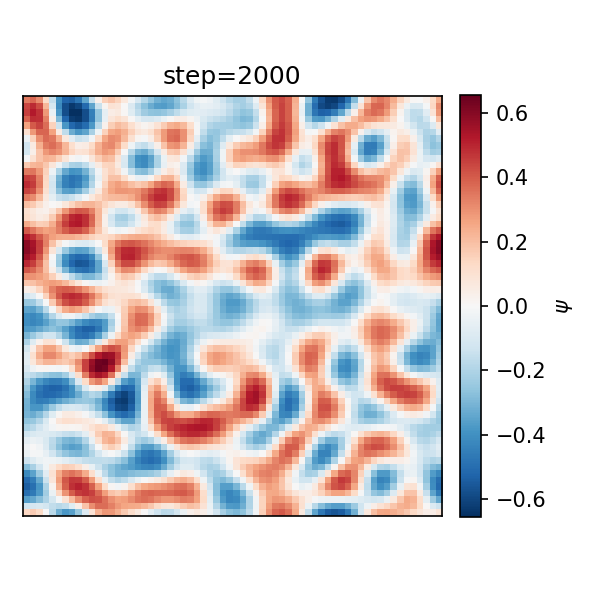
\includegraphics[width=0.32\textwidth]{figures/cahn-hilliard/early.png}\hfill
  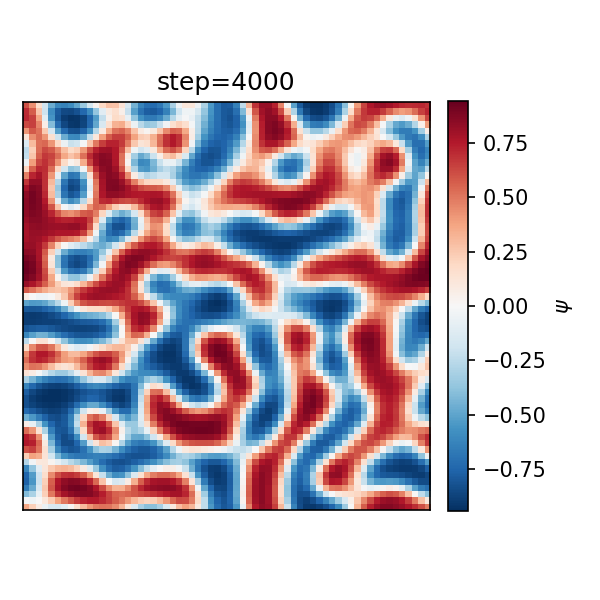
\includegraphics[width=0.32\textwidth]{figures/cahn-hilliard/mid.png}\hfill
  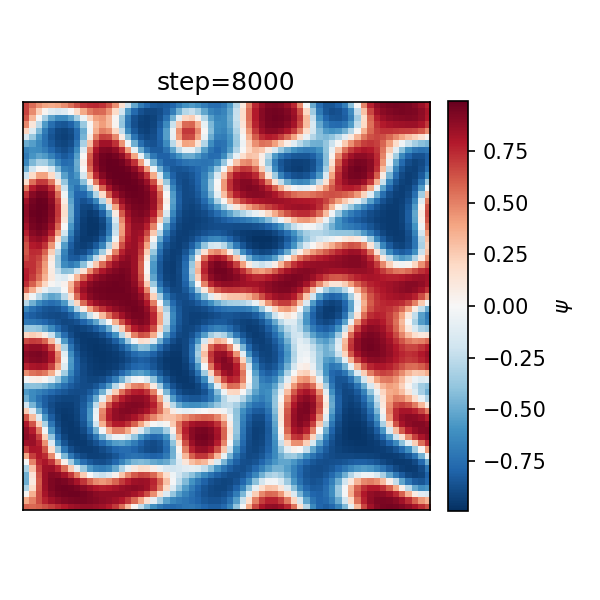
\includegraphics[width=0.32\textwidth]{figures/cahn-hilliard/late.png}
  \caption{$z$-midplane slices of $\psi$ from a $64^3$ Cahn--Hilliard
  run with $M=\kappa=1$, seed $42$, $\Delta x=1$, $\Delta t = 0.01$.
  Left ($t=20$): post-spinodal regime, $|\psi|$ has not yet saturated
  to the equilibrium amplitude. Center ($t=40$): bicontinuous
  two-phase pattern with sharp interfaces and $|\psi|\approx 1$. Right
  ($t=80$): coarsened domains, same amplitude. The reproduction of
  this textbook coarsening sequence is the qualitative-acceptance
  evidence for Phase 12.}
  \label{fig:ch-coarsening}
\end{figure}

The gradient energy
\(E_{\text{grad}} = \int |\nabla\psi|^2\,\dd V\) is a useful coarse
proxy for inverse domain size. In the default run it peaks near
\(t\approx 30\) (interfaces fully formed, smallest typical domains)
and decreases monotonically afterward. The Phase 12 acceptance test
\passthrough{\lstinline!CahnHilliardCoarseningRun.MonotoneCoarsening!}
locks in this property in CI on a smaller (24\(^3\), \(\kappa=0.5\))
budget-friendly run.

\subsection{What this does \emph{not} do}\label{phase12-not-do}

\begin{itemize}
\tightlist
\item
  \textbf{Implicit / IMEX time stepping.} The explicit
  \(\Delta t \sim h^4\) bound is brutal and grows worse with
  resolution. A semi-implicit treatment of the
  \(-M\kappa\nabla^4\psi\) term arrives in Phase 19 alongside the
  matrix-free linear-solver scaffolding.
\item
  \textbf{Non-periodic boundary conditions.} The demo runs purely on
  Phase 1's periodic \passthrough{\lstinline!IndexPolicy::Periodic!}.
  Dirichlet / Neumann at Phase 18 will let the same setup model a CH
  system with no-flux walls.
\item
  \textbf{\(R(t)\sim t^{1/3}\) quantitative scaling fit in CI.} The
  Phase 12 acceptance bar is qualitative (visual + monotone-coarsening
  programmatic check). A separately-runnable scaling benchmark could
  be added later.
\item
  \textbf{Vector- or tensor-valued CH.} Multi-component CH (model B
  for binary alloys with a multi-component order parameter) and model
  H (CH coupled to fluid flow) belong with Phase 13 / 14.
\end{itemize}

For the dispersion-relation derivation, the
\(\sigma(\mathbf k)\,\Delta t\le 2.7853\) RK4 stability argument, and
the rejected alternatives, see the ``Cahn--Hilliard demo'' chapter of
the Developer Note.

\chapter{Vector and tensor fields}
\label{chap:vector-tensor-fields}

\begin{quote}
Spec dir:
\passthrough{\lstinline!specs/2026-05-04-phase-13-vector-tensor-fields/!}.
Version: \passthrough{\lstinline!0.13.0!}.
\end{quote}

\subsection{What this gives you}\label{phase13-what}

\passthrough{\lstinline!Field<T>!} now instantiates with a rank-2
tensor element, and the rank-raising / rank-lowering arithmetic
identities work as expected. Three new public symbols:

\begin{itemize}
\tightlist
\item
  \passthrough{\lstinline!gridcalc::core::Mat3d!} — alias for
  \passthrough{\lstinline!Eigen::Matrix3d!} (standard Eigen module).
  Lives in
  \passthrough{\lstinline!core/EigenAliases.hpp!} alongside
  \passthrough{\lstinline!Vec3d!}.
\item
  \passthrough{\lstinline!diff::gradient(Field<Vec3d>) -> Field<Mat3d>!} —
  rank-raising gradient with the convention
  \(M(i, j) = \partial_j v_i\).
\item
  \passthrough{\lstinline!diff::divergence(Field<Mat3d>) -> Field<Vec3d>!} —
  rank-lowering divergence with the matched convention
  \((\mathrm{div}\,M)_i = \partial_j M(i, j)\).
\end{itemize}

Plus the contraction primitives in the new
\passthrough{\lstinline!tensor/Contraction.hpp!}:

\begin{itemize}
\tightlist
\item
  \passthrough{\lstinline!tensor::trace(Field<Mat3d>) -> Field<double>!}
\item
  \passthrough{\lstinline!tensor::singleContract(Field<Mat3d>, Field<Mat3d>) -> Field<Mat3d>!}
  — pointwise matrix product \((A \cdot B)(i,j) = A(i,k)\,B(k,j)\).
\item
  \passthrough{\lstinline!tensor::doubleContract(Field<Mat3d>, Field<Mat3d>) -> Field<double>!}
  — pointwise full contraction \(A : B = A(i,j)\,B(i,j)\).
\end{itemize}

\textbf{Out of scope at Phase 13.}
\passthrough{\lstinline!Field<Tensor3>!} and
\passthrough{\lstinline!Field<Tensor4>!} (rank-3 and rank-4 tensor
fields) are deferred to Phase 15, where the contraction
expression-template work that motivates them lands together. The
unsupported-Eigen-tensor-module portability question stays deferred.

\subsection{Index conventions}\label{phase13-conventions}

The rank-2 gradient stores
\(M(i, j) = \partial_j v_i\): row index \(i\) selects the vector
component being differentiated; column index \(j\) selects the
derivative axis. Under this convention the trace recovers the
divergence,
\[
\mathrm{tr}(M) = \partial_x v_x + \partial_y v_y + \partial_z v_z = \nabla\cdot v,
\]
and the matched rank-2 divergence
\((\mathrm{div}\,M)_i = \partial_j M(i, j)\) gives the natural vector
Laplacian under composition:
\[
\big(\mathrm{div}(\nabla v)\big)_i = \partial_j \partial_j v_i = (\nabla^2 v)_i.
\]

\subsection{API}\label{phase13-api}

The Phase 2 scalar gradient and divergence keep their existing
signatures unchanged; Phase 13 adds new overloads on
\passthrough{\lstinline!Field<Vec3d>!} and
\passthrough{\lstinline!Field<Mat3d>!} respectively. Both new
overloads inherit the Phase 7
\passthrough{\lstinline!Order!} template parameter (default
\passthrough{\lstinline!2!}; \passthrough{\lstinline!4!}-th order
available):

\begin{lstlisting}[language={C++}]
namespace gridcalc::diff {

template <int Order = 2>
core::Field<core::Mat3d> gradient(const core::Field<core::Vec3d>& field);  // new

template <int Order = 2>
core::Field<core::Vec3d> divergence(const core::Field<core::Mat3d>& mfield);  // new

}  // namespace gridcalc::diff

namespace gridcalc::tensor {

core::Field<double>      trace(const core::Field<core::Mat3d>& mfield);
core::Field<core::Mat3d> singleContract(const core::Field<core::Mat3d>& a,
                                        const core::Field<core::Mat3d>& b);
core::Field<double>      doubleContract(const core::Field<core::Mat3d>& a,
                                        const core::Field<core::Mat3d>& b);

}  // namespace gridcalc::tensor
\end{lstlisting}

\subsection{Worked example: three vector
identities}\label{phase13-identities}

The Phase 13 acceptance test
(\href{../../../test/vector_tensor_test.cpp}{\passthrough{\lstinline!test/vector\_tensor\_test.cpp!}})
verifies three identities programmatically.

\subsubsection{1. Hessian symmetry
(\(\nabla\times\nabla\phi = 0\))}\label{phase13-hessian}

For smooth \(\phi\), the Hessian \(\nabla\nabla\phi\) is symmetric.
Composed Phase 2 gradients realize the rank-raising version directly:

\begin{lstlisting}[language={C++}]
Field<double> phi(grid, [](double x, double y, double z) {
    return std::sin(x) * std::cos(y) * std::sin(z);
});
auto H = gradient(gradient(phi));  // Field<Vec3d> -> Field<Mat3d>

// Each H(i, j, k) is symmetric to round-off:
EXPECT_NEAR(H(7, 11, 5)(0, 1), H(7, 11, 5)(1, 0), 1e-12);
\end{lstlisting}

The agreement is to round-off (not stencil-order tolerance) because
the FD operators \(\partial_i\) and \(\partial_j\) commute on a
periodic uniform grid.

\subsubsection{2.
\(\mathrm{tr}(\nabla v) = \nabla\cdot v\)}\label{phase13-trace}

\begin{lstlisting}[language={C++}]
auto v = sampleVectorField(grid, [](double x, double y, double z) {
    return Vec3d(std::sin(x) * std::cos(y),
                 std::sin(y) * std::cos(z),
                 std::sin(z) * std::cos(x));
});
auto trace_grad_v = tensor::trace(diff::gradient(v));
auto div_v        = diff::divergence(v);
// trace_grad_v == div_v to round-off pointwise.
\end{lstlisting}

\subsubsection{3. \(\nabla\cdot(\nabla v) = \nabla^2
v\)}\label{phase13-vec-laplacian}

For the same \(v\), each Cartesian component depends on exactly two
axes, so its scalar Laplacian sums two
\(-\text{component}\) contributions and the vector Laplacian is
\(\nabla^2 v = -2\,v\). The composition
\passthrough{\lstinline!divergence(gradient(v))!} is a stride-2
second-derivative stencil (the same composed-stencil phenomenon
documented for \passthrough{\lstinline!divergence(gradient(\(\psi\)))!} versus
\passthrough{\lstinline!laplacian(\(\psi\))!} in Phase 2's note); it converges
to the analytical \(\nabla^2 v\) at \(\mathcal{O}(h^2)\) but with a
different leading-error constant than
\passthrough{\lstinline!diff::laplacian!} applied componentwise. The
test checks the rate against the closed-form
\(-2\,v\), not against a discrete componentwise Laplacian.

\subsection{What this does \emph{not} do}\label{phase13-not-do}

\begin{itemize}
\tightlist
\item
  \textbf{Rank-3 / rank-4 tensor fields.} Deferred to Phase 15.
\item
  \textbf{Expression-template contraction layer.} Deferred to Phase 15
  alongside the
  \passthrough{\lstinline!func::evaluate!}-over-tensor-fields surface
  that motivates it.
\item
  \textbf{Explicit \texttt{curl} operator.} The
  \passthrough{\lstinline!gradient(gradient(phi))!}-symmetry test
  discharges the
  \(\nabla\times\nabla\phi = 0\) identity in rank-raising
  vocabulary; an explicit
  \passthrough{\lstinline!curl!} (rank-1 \(\to\) rank-1) is not on
  the roadmap and is not added speculatively.
\item
  \textbf{Vector / tensor spectral cross-check.} The Phase 9 fixture
  parameterizes over scalar-input FD operators; the rank-raising
  variants are not (yet) in its scope.
\end{itemize}

For the construction of the manufactured solutions and the rate
arguments, see the ``Vector and tensor fields'' chapter of the
Developer Note.

\chapter{Diamond-lattice example}
\label{chap:diamond-lattice}

\textit{Placeholder. The diamond-lattice multi-atom-basis example
chapter is a deliverable of Phase 17; this stub reserves the chapter
slot.}


% --- Back matter --------------------------------------------------------------

\backmatter

\chapter*{License}

Proprietary. All rights reserved. Redistribution requires authorization
from the project owner. See the repository's \path{LICENSE} file.

\end{document}
